%%%%%%%%%%%%%%%%%%%%%%%%%%%%%%%%%%%%%%%%%%%%%%%%%%%%%%%%%%%%%%%%%%
%%%%%%%% ICML 2013 EXAMPLE LATEX SUBMISSION FILE %%%%%%%%%%%%%%%%%
%%%%%%%%%%%%%%%%%%%%%%%%%%%%%%%%%%%%%%%%%%%%%%%%%%%%%%%%%%%%%%%%%%

% Use the following line _only_ if you're still using LaTeX 2.09.
%\documentstyle[icml2013,epsf,natbib]{article}
% If you rely on Latex2e packages, like most moden people use this:
\documentclass{article}

% For figures
\usepackage{graphicx} % more modern
%\usepackage{epsfig} % less modern
\usepackage{subfigure} 

% For citations
\usepackage{natbib}

% For algorithms
\usepackage{algorithm}
\usepackage{algorithmic}
\usepackage{amsmath}

% As of 2011, we use the hyperref package to produce hyperlinks in the
% resulting PDF.  If this breaks your system, please commend out the
% following usepackage line and replace \usepackage{icml2013} with
% \usepackage[nohyperref]{icml2013} above.
\usepackage{hyperref}

% Packages hyperref and algorithmic misbehave sometimes.  We can fix
% this with the following command.
\newcommand{\theHalgorithm}{\arabic{algorithm}}

% Employ the following version of the ``usepackage'' statement for
% submitting the draft version of the paper for review.  This will set
% the note in the first column to ``Under review.  Do not distribute.''
%\usepackage{icml2013}
% Employ this version of the ``usepackage'' statement after the paper has
% been accepted, when creating the final version.  This will set the
% note in the first column to ``Proceedings of the...''
 \usepackage[accepted]{icml2013}

% The \icmltitle you define below is probably too long as a header.
% Therefore, a short form for the running title is supplied here:
\icmltitlerunning{Predicting Stock Trends Using Financial News Articles}

\begin{document} 

\twocolumn[
\icmltitle{6.867 Final Project: Predicting Stock Trends\\
            Using Financial News Articles}

% It is OKAY to include author information, even for blind
% submissions: the style file will automatically remove it for you
% unless you've provided the [accepted] option to the icml2013
% package.
\icmlauthor{Keren Gu}{kgu@mit.edu}
\icmlauthor{Ernest Zeidman}{zeidman@mit.edu}

% You may provide any keywords that you 
% find helpful for describing your paper; these are used to populate 
% the "keywords" metadata in the PDF but will not be shown in the document
\icmlkeywords{boring formatting information, machine learning, ICML}

\vskip 0.3in
]


\section{Introduction}


There have been many efforts to apply machine learning to the forecasting of financial time series data. For example it is possible to apply support vector machines (SVMs) to historical prices to forecast price movement; In fact, SVMs perform this task better than back propagated neural networks [1]. There have also been more varied approached, including the application of microblogging signals. It is possible to predict the direction of the NASDAQ by analyzing 1\% of all tweets [2]. Alternatively its possible to make weak predictions about a particular stock using the feed of tweets mentioning the company name or ticker [3].

Our aim is to investigate how news articles can be used to predict the direction of stock movement. We investigate the predictive power of one article at a time, asking whether an article about company X released today can be used to forecast whether stock X will go up or down during the next day. In spirit, the problem is about sentiment analysis. It is based on the idea that investors will make trading decisions based on the tone and content of the news they read. However, the sentiment analysis is implicit because our labels (stock price changes) don't directly describe the article sentiment. The main goal of the project is to find a support vector machine, which performs this classification task. We also look into two alternative approaches, using regression and using a naive Bayes classifier.

It is worth noting that predictive power is not the full story in financial forecasting. Consider the trading strategy which buys when the classifier forecasts a positive movement and shorts when the classifier forecasts a negative movement. Such a strategy can have a negative expected value even if it makes money most days (e.g. if when it is wrong, it is terribly wrong).

All scripts, data-files, experiments, and results of this project can be found at this repository: \texttt{http://bit.ly/1eTPikL} . 

\section{Approaches}



\subsection{Data Collection}
We collected two types of data for this project: articles and corresponding labels. 

We first selected a set of 31 largest technology companies from NASDAQ and collected all news article by scraping each company's `news' section on Google Finance. The available set of news articles span exactly 2 years into the past with majority of the articles published from the past month. We selected all of our articles from Reuter's Key Development in order to keep our articles uniformly distributed over the past 2 years. In total, we collected 1737 articles for 31 companies over 2 years. 

In order to generate labels for the obtained articles, we looked at the prices for the company of interest around the time the article is published, under the assumption that the sentiment of the article is reflected in the stock's price in the near future. While only daily prices are available on the web, the set of prices that we collected contains the closing price on the day of publishing, the opening price on the next day, and the closing price of the next day. Together, these daily prices form 3 sets of labels: (i) after-day-label, defined as the after-hours price change; (ii) next-day-label, defined as the price change on the day after the article was published; and (iii) combined-label, defined as the sum of the after-day-label and next-day-label.

In the case where multiple articles are collected on the same day for the same company, we merge the feature vectors of these articles into one. Because with labels representing the price-change over a day, we have no way of distinguishing the fraction of price change that is caused by one article over another. After merging, we have 1477 articles with distinct company and date combination. 

Lastly, the type of content collected is mainly announcements, summaries of news reports on company earning or dividends. All articles are very formal and highly objective. The following is an excerpt from a random article: 

{\em``International Business Machines Corp announced that Australian fruit and vegetable retailer Harris Farm Markets has selected an IBM Flex System solution to help support its business growth and reduce IT costs and complexity."}


\subsection{SVM}

The main approach to the classification problem is the application of a support vector machine. A SVM finds a hyperplane which bisects the input space into two halves corresponding with two classes. This hyperplane has the maximal margin, meaning it is as far as possible from all training points. If the sample points aren't linearly separable, it may be necessary to project them into a feature space. The radial basis kernel, which we employ, generates a feature space which is always linearly separable. 

Stock price movements are characteristically noisy and erratic, meaning that our labels have a fair measure of noise. Basic SVMs can be very fragile and thrown off by a single mislabeled point. To mitigate this we employ slack variables, which allow some of the training points to slide into margin or even to be misclassified. Consequently our SVM has two parameters which need to be tuned: $C$ governs the relative penalty given to the use of slack variables for each point, $\xi_i$, which is apparent in the primal form of the optimization problem:

$$ \min \frac{1}{2}\|\theta\|^2 + C \sum_i \xi_i$$

The other parameter, $\beta$, comes into play when using the radial basis kernel. $\beta$ governs the relative ``distance" between points. For the major part of our project, we employed the radial basis kernel:

$$K(x, x') = \exp \big ( - \dfrac \beta 2 ||x-x'||^2 \big ), \ \beta > 0$$

Larger $\beta$ means that even adjacent points are treated as if they are unrelated. 

We used MATLAB's implementation of the \texttt{trainsvm} and \texttt{svmclassify}. MATLAB's \texttt{trainsvm} uses the Sequential Minimal Optimization (SMO) method as its default method to identify the support vectors $s_i$, weights $\alpha_i$, and bias $b$ that are used to classify a vector $x$ according to the following equation: 

$$\text{sign}\big\{\sum_i\alpha_i K(s_i, x) + b\big\}$$ 

where $K(x, x')$ is the kernel function of choice. We also experimented with the Quadratic Programming method, which is documented to give more precise solutions, though slower in performance. 

\texttt{trainsvm} also allows us to set the tolerance with which the Karush-Kuhn-Tucker (KKT) condition is checked when using the SMO method. This parameter also serves as a restraint on the minimal value of $C$ that can be set. The default value is set as $10^{-3}$. We experimented a little with this parameter when trying out the linear kernel on one of our feature variants. In addition, \texttt{trainsvm} also allows us to set the percentage of dataset that is allowed to violate the KKT condition. We kept this parameter as 0.

To compare and verify the setup of MATLAB's \texttt{trainsvm}, we trained and compared results against the implementation from Problem Set 6. 

\subsection{Regression}

We applied our regression implementation from Problem Set 3 to our dataset to investigate whether we can extract useful information from the magnitude of price changes (the SVM only considers the sign of the price changes). Since the feature space is so large, we employ regression with regularization, optimizing:

$$\frac{\lambda}{2}\|\theta\|^2 + \frac{1}{2} \sum_i (y_i - \theta \cdot \phi(x_i) - \theta_0)^2 $$

The regression model gives more fine-grained predictions, allowing more complex trading strategies. For example consider the strategy which buys or shorts an amount which is proportional to the magnitude of the prediction. The idea here is that since regression intrinsically penalizes large deviations, it may induce risk-mitigating trading strategies.

\subsection{Naive Bayes}

We applied a basic naive Bayes classifier (NBC) to our dataset to give a benchmark against which we can compare our SVM. A naive Bayes classifier works by finding the class which has the highest probability conditioning on the observed inputs. The NBC assumes that every document is produced from a mixture model and that given a document and its class, the words in the document are generated independently from each other. To compute the probability of a document belonging to a class, the NBC uses the Bayes rule as follows: 

$$P(c_j|D) = \dfrac{P(c_j)\Pi_i P(w_i|c)}{P(D)}$$

, and makes a classification by computing 

$$\text{argmax}_{c_j} P(c_j) \Pi_i P(w_i|c)$$

. The naive Bayes method is a very fast way to generate a decent linear classifier. 

\section{Features}

We investigated several variations on feature representations of articles. The primary representation of an article is a ``bag of words", represented by a vector of word counts. We investigated whether it would be beneficial to discard the most frequent or the most infrequent words; or to include a couple other derived features. For comparison, we tried a feature representation based on historical prices. The specific feature representations are given below.

\subsection{Standard Feature Representation} 
We consider all the 7358 English words that occur in our corpus of articles. Each article is represented by a vector $v$, where $v_i$ gives the number of occurrences of word $i$ in the title and body.

\subsection{Feature Variant 1 (V1)}
We eliminate the 2299 words which only occur once. The intuition behind this variant is that when we split our dataset into training and testing set, these words either do not contribute to the training or are not useful when being classified. Overall, these words do not contribute to lowering the generalization error. 

\subsection{Feature Variant 2 (V2)}
We eliminate the 10\% of words which are the most frequent. (These are words which occur 28 times or more). The intuition behind this variant is that the most frequent words are likely to be articles and neutral words that have no sentiment. 

\subsection{Feature Variant 3 (V3)}
Each article is represented by the following features: (1) the time of the day the article is published, (2) the day of the week the article is published, (3) the length of the article in characters, (5) the number of words in the title, (6) the number of words in the body, (7) the number of numbers and symbols in the article, (8) the average word length of the article, (9) the sum of positive scores of all words in the article, and (10) the sum of negative scores over all words in the article, where the positivity and negativity values of each English word is obtained from SentiWordNet. 

\subsection{Feature Variant 4 (V4)}
For each article, we include the opening, closing, high, and low prices, as well as the transaction volume for each of the 20 trading days before the day in which an article is released, a total of 100 features per article. The goal of this variant is to compare how a company's performance in the past month reflects the after-day price changes against how articles reflect the after-day price changes . 


\subsection{Combined Feature Representation 1 (C1)}
This is the concatenation of feature variant 3 and feature variant 4. 

\subsection{Combined Feature Representation 2 (C2)}
This is the concatenation of the standard representation and variant 4.\\

Another representation that we considered but did not pursue is bigram-representation of the article, where every two consecutive words is considered as a feature. The reason we did not pursue this is because of the already large feature space relative to the number of training points that we have. In addition, upon careful examination of the content of the articles that we have collected, as presented in section 2.1, the articles are direct and objective. There isn't much negation, nor many instances of complex tone (e.g. sarcasm).

\section{Results}

All the results reported below come from using after-day-labels. We also tried next-day-labels and combined-labels, but found across the board that articles have a diminished ability to forecast these. This makes sense, because next-day-labels and combined-labels extend further into the future.

\subsection{K-Fold Cross Validation (KFCV)}
Initially to test our model, we implemented \texttt{split\_data} which randomly permutes the dataset and partitions it into training and test sets. We tested our model by training and testing on different splits of the input data and averaging over the error rates. 

However, in order to compare different models against each other and against different feature representations, we implemented \texttt{KFCV}, which is actually a K-fold cross validation, where we divide the entire dataset into K blocks where each block is left out during each iterations while the remaining K-1 blocks are used as the training set. We made this modification so that each experiment could finish in a reasonable amount of time. Throughout this project, K has been selected as 18. 

\subsection{SVM}

\begin{figure}[t]
\vskip 0.2in
\begin{center}
\centerline{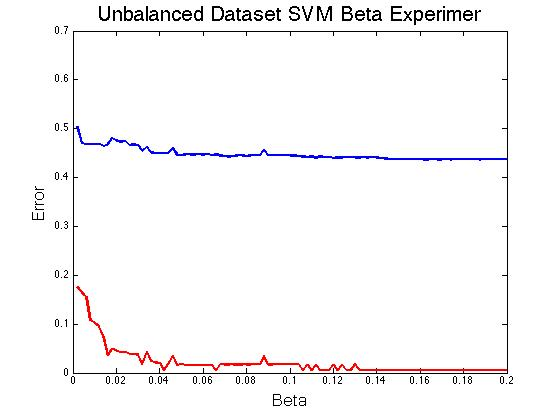
\includegraphics[width=\columnwidth]{beta_experiment.jpg}}
\caption{The training error (red) and testing error (blue) of SVM with fixed $C=1$ and $\beta$ varying from $0.001$ to $0.2$ using the standard features. For values of $\beta$ greater than $0.2$, the error rate converges to $43.47\%$.}
\label{beta-experiment}
\end{center}
\vskip -0.3in
\end{figure} 


\begin{table}[b]
\caption{SVM Training and Generalization Error Over All Feature Representation Variant Performances}
\label{svm-feature-experiment}
\vskip 0.15in
\begin{center}
\begin{small}
\begin{sc}
\begin{tabular}{lcccr}
\hline
\abovespace\belowspace
Variant & Train & Test & $\beta^*$ & $C^*$ \\
\ & Error & Error \\
\hline
\abovespace
Standard     & 1.69\% & 48.06\% & .0120 & .0500\\   % Beta already doubled.
Variant 1    & 0.32\% & 48.29\% & .0120 & 1.000\\
Variant 2    & 4.60\% & 48.29\% & .0600 & 2.000\\
Variant 3    & 42.60\% & {\bf47.07}\% & .0400 & 1.000\\
Variant 4    & 30.32\% & 47.37\% & .0800 & 2.000\\
Combined1    & 43.85\% & 50.19\% & .0020 & 1.000\\
\belowspace
Combined2    & 0.15\% & 49.20\% & .0140 & 1.000\\
\hline
\end{tabular}
\end{sc}
\end{small}
\end{center}
\vskip -0.1in
\end{table}

In our first attempt at using a SVM, we used the standard feature representation of the entire 1737 articles that we collected, the radial basis kernel and, and default values of $C=1$ and $\beta=1$. We obtained the generalization error of 43.47\% from our K-fold cross validation. 

We varied our parameters in order to find the values of $C$ and $\beta$ that would lower the generalization error by fixing one value and varying the other. The result of fixing $C=1$ and varying $\beta$ over the interval of $[0.001, 0.2]$ is shown in Figure~\ref{beta-experiment}. We also experimented with $\beta$ up to 10, and the result shows that the generalization error for $\beta\geq 0.1$ converges to 43.47\%. In addition, we fixed $\beta$ and varied $C$ over the interval of $[0.01, 1000]$ and found that for any $C\geq 1$, the generalization error is 43.47\%. We also see that the training error for when $\beta\geq 3$ and $C\geq1$ is smaller than $0.003$.  

This result is contrary to what is expected, and is a clear example of overfitting. Upon further investigation, by looking at the distribution of positive and negative after-day-labels and by looking at the average number of false-positive and false-negative classifications, we found that the fraction of negative points in our dataset is 43.52\%, and that the SVM is making 99\% positive classifications. (Though the 1\% negative classification has greater than 99\% accuracy.) This led us to balance our dataset to obtain 1304 articles with balanced labelings. 


\begin{figure}[hb]
\vskip 0.1in
\begin{center}
\centerline{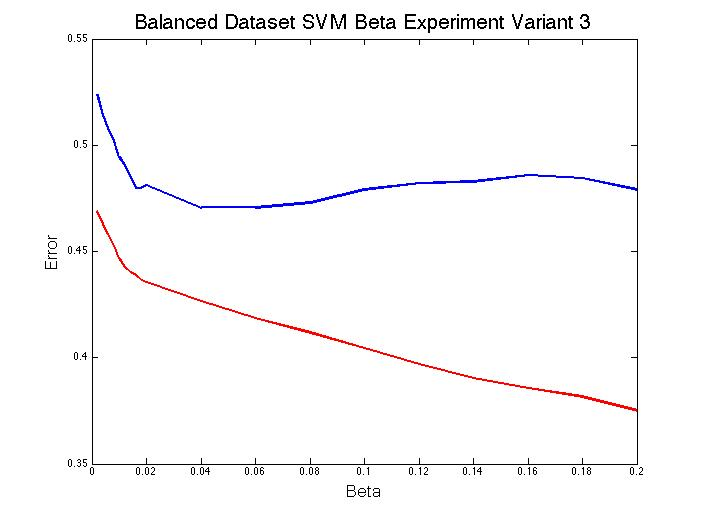
\includegraphics[width=\columnwidth]{beta_experiment_feat_v3.jpg}} 
\caption{The training error (red) and testing error (blue) of SVM with fixed $C=1$ and $\beta$ varying from $0.001$ to $0.2$ using Feature Variant 3. For values of $\beta$ greater than $0.2$, the training errors continues to decrease and the generalization error increases to 51.11\% at $\beta=10$.}
\label{feat-v3-experiment}
\end{center}
\vskip -0.2in
\end{figure} 


After balancing our dataset, we ran two experiments over every feature mentioned in the previous section in order to find the best values of $\beta$ and $C$. In each of our experiments, we fixed one and varied the other, and used KFCV to assess our training and testing errors. Specifically, to find the optimal value of $\beta$ for each feature variant, we fixed $C=1$ and iterated over 37 values of $\beta$ ranging from 0.001 to 20. To find the optimal value of $C$, we fixed $\beta$ for each feature variant as the optimal value we found in the previous experiment and iterated over 28 values of $C$ ranging from 0.01 to 10. The resulting best values of $\beta$ and $C$ and their corresponding test and training error for each feature variant is shown in Table~\ref{svm-feature-experiment}. 


Unlike the result from using the imbalanced dataset, the generalization error as a function of varying $\beta$ with a fixed $C=1$ shows a healthy global minimum at $\beta=\beta^*$, and the training error decreases as we increase $\beta$. A sample plot of the training and test error for feature variant 3 is shown in Figure~\ref{feat-v3-experiment}. 

In addition, we also considered linear kernels for a number of feature variants (S, V3, V4, and C1). We explored $C$ values ranging from $0.001$ up to $1$. For small values of $C$, we needed to adjust the tolerance at which the KKT condition was checked. For large values of $C\geq0.8$, when using the standard feature variant, we found it necessary to increase the maximum number of iterations allowed while using the Quadratic programing method. The best $C$ value for each variant and their corresponding training and K-fold cross validation errors are shown in Table~\ref{linear-svm}. 

When working with the standard feature set, the number of features is the number of distinct English words in the entire dataset, which was 7358. Since the VC-dimension of a $k$-dimension linear classifier is greater than $k$ and our entire dataset after balancing and merging consists of 1304 articles, we know it is possible to generate a model with zero training error. However, we are using slack variables so we get slightly increased error of 0.07\%
. Feature variants 3 and 4, on the other hand, have much smaller feature spaces, which explains the large training error from using the linear kernel.

Among all the feature variants, we expected feature variants 3 and 4 to do well. Specifically, the positive and negatives scores in feature variant 3 should be a good indicator of the sentiment of the article. And if our assumptions are correct, the sentiment of an article should be a good indicator of the stock's price change. Feature variant 4 was expected to do well based on previous research mentioned in the Introduction section. In addition, we expected the combined feature 1 to perform the best, combining two of the best performing feature variants can, at worst, give a equally performing classifier. However in practice, the result showed a worse performance of $50.19\%$ error. Since the lowest test errors for variants 3 and 4 are found with different values of $\beta$ and $C$, we can not make this a strict comparison with the combined feature. We also consider the possibility that SVM optimized for a greater margin, but did not generalize well when tested with our K-fold cross validation. 


\begin{table}
\caption{Linear SVM using Selected Feature Representation Variants}
\label{linear-svm}
\vskip 0.15in
\begin{center}
\begin{small}
\begin{sc}
\begin{tabular}{lccc}
\hline
\abovespace\belowspace
Variant & Train Error & Test Error & $C^*$ \\
\hline
\abovespace
Standard     & 0.44\% & 49.17\% & 1\\
Variant 3    & 46.71\% & 50.33\% & .5000\\
Variant 4    & 46.28\% & 49.25\% & .0050\\
Combined1    & 42.70\% & 49.00\% & 1\\
\hline
\end{tabular}
\end{sc}
\end{small}
\end{center}
\vskip -0.1in
\end{table}



%\subsection{Feature Comparisons}

%We performed a seveweay experiment to determine the best feature representation. In each case we used KFCV with the parameters that we found earlier (i.e. $\beta = 3$ and $C = 1$). The results of the experiment are visible in Table~\ref{feature-variants}, which shows that the standard feature representation achieves the lowest test error of $43.54\%$. Interestingly, it also shows that you do just as well if you eliminate all the single occurrence words.



\subsection{Regression}

We performed two experiments to find optimal parameterization for $\beta$ and $\lambda$ for all seven feature variants. First we fixed $\lambda$ at 1, while varying $\beta$ over 37 values. Then using the optimal  $\beta$ values, we iterated over $28$ values of $\lambda$. In both cases we pick the parameterization that leads to the smallest KFCV test error when using the regression model to make directional predictions. Variant 3 performs best as is evident
in Table~\ref{reg-feature-experiment}.

We expected the regression model to have similar results to the SVM because their optimization problems are so similar. In fact, the results are generally comparable in terms of testing error. The exception seems to be feature variant 4, which performs much worse with a regression model. At the same time, the regression model for V3 achieves our overall best performance with a test error of $46.54\%$, beating the best SVM by a small margin. One explanation is that a regression model gets more information from real-valued labels, than SVM models get from single bit labels.

\begin{table}[b]
\caption{Regression Training and Generalization Error Over All Feature Representation Variant Performances}
\label{reg-feature-experiment}
\vskip 0.15in
\begin{center}
\begin{small}
\begin{sc}
\begin{tabular}{lcccr}
\hline
\abovespace\belowspace
Variant & Train & Test & $\beta^*$ & $\lambda^*$ \\
\ & Error & Error \\
\hline
\abovespace
Standard     & 0.07 \% & 47.98\% & 0.18 & 0.01\\ % beta already doubled, dont redouble because that leads to quadrupling 
Variant 1    & 0.07 \% & 47.98\% & 0.18 & 0.07\\ 
Variant 2    & 4.56 \% & 49.09\% & 0.18 & 0.005\\ 
Variant 3    & 1.02 \% & {\bf46.53\%} & 0.004 & 0.005\\ 
Variant 4    & 0 \% & 54.14\% & 0.002 & 0.005\\ 
Combined1    & 0 \% & 54.14\% & 0.002 & 0.005\\ 
\belowspace
Combined2    & 0.31 \% & 49.95\% & 0.12 & 0.01\\ 
\hline
\end{tabular}
\end{sc}
\end{small}
\end{center}
\vskip -0.1in
\end{table}


\subsection{Naive Bayes}
We tested the effectiveness of the naive Bayes classifier by using K-fold cross validation on all seven of the feature variants. It performs worse than the support vector machine across the board. The generated models reveals that ``billing", ``increases", and ``proposes" are very positive words; that ``extreme" and ``disclosing" are very negative. However the predictive strength of these words is uncertain given the high observed testing error. The results are in Table~\ref{nbc-results}.

\begin{table}[t]
\caption{NBC Feature Representation Variant Performances}
\label{nbc-results}
\begin{center}
\begin{small}
\begin{sc}
\begin{tabular}{lcccr}
\hline
\abovespace\belowspace
Variant & Train Error & Test Error \\
\hline
\abovespace
Standard    & 17.11\% & 50.02\% \\
Variant 1    & 18.61\% & 50.09\% \\
Variant 2    & 14.40\% & 52.00\% \\
Variant 3    & 49.08\% & 53.54\% \\
Variant 4    & 49.79\% & 49.80\% \\
Combined1    & 49.41\% & 51.01\% \\
\belowspace
Combined2    & 17.10\% & 50.31\% \\
\hline
\end{tabular}
\end{sc}
\end{small}
\end{center}
\vskip -0.3in
\end{table}


\section{Discussion}

% Our assumptions
The ideation of this project is based on the assumption that the price change of a company's stock is caused by the news and announcements made about the company on the day of or day before. Realistically, many causal factors impacting asset movements. Also, even if news articles have a large role in investor decisions, so do expectations. For instance, an article with a positive announcement may discourage an investor if its not as positive as expected. In light of this complicated environment, we think the $47.07\%$ achieved by variant 3 is pretty good considering two major limitations: the lack of training data and extremely noisy labels. (As a comparison, testing our SVM on a random labeling gave us 51\%.) Furthermore, we think it is very noteworthy that the the derived article features (V3) have as much predictive power as the historical prices (V4). This suggests that news articles can be an important signal in financial decision making.

% Problem 1: Not enough articles. 
Finding news articles going 2 years back was a limiting factor mainly due to the fact that news becomes archived after a short amount of time. This introduced a problem for us: when the number of features is greater than the size of the training set, we cannot say anything about the test error because the bound on the generalization error (with probability at least $1-\delta$), 
$$ R(h) \leq R_n(h) + \sqrt{\dfrac{h(\log(\frac{2N}h)+1)-log(\frac \delta 4)}{2N}}$$

where $h=\text{VC}(\mathcal{H})$ only holds when $h\ll N$. The same reason explains that when the linear kernel is used to classify the standard feature variant, the separater did no learning yet it was able to separate more than 99\% of the training point correctly. 

To possibly reduce the difference between the size of our training set and the size of our feature space, in feature variants 1 and 2, we eliminated 30\% and 10\% of our features respectively and found no improvement in the generalization error. This lack of improvement could still be due to our limited number of articles. In order to obtain much larger number of financial news articles related to a set of companies, we would imitate some existing research and collect our data over longer period of time, scraping news on a daily or weekly basis. 

% Problem 2: Labels are too noisy.
Our second limitation was due to the lack of accurate labels. While we collected after-day and next-day price changes, a number of other factors could be better indicators of the price change. For instance, if the article is released earlier in the trading day, the effect on the market may have been taking into account 30min after the release; or the price change could have been caused by a more global news event. A possible solution is to gain access to intra-day price change. Then, we could label each article by the price change 30 minutes or an hour after the release of the article. This will allow us to generate labels that are more finely tuned, and that are better representations of the articles. 


\section{References}

[1] Kyoung-jae Kim, Financial time series forecasting using support vector machines, Neurocomputing, Volume 55, Issues 1–2, September 2003, Pages 307-319, ISSN 0925-2312.

[2] Xue Zhang, Hauke Fuehres, Peter A. Gloor, Predicting Stock Market Indicators Through Twitter “I hope it is not as bad as I fear”, Procedia - Social and Behavioral Sciences, Volume 26, 2011, Pages 55-62, ISSN 1877-0428.

[3] E. J. Ruiz, V. Hristidis, C. Castillo, A. Gionis, and A. Jaimes.
Correlating financial time series with micro-blogging
activity. In Proc. of the 5th ACM International Conference
on Web Search and Data Mining, WSDM ’12, pages
513–522, Seattle, WA, 2012.


\end{document} 


% This document was modified from the file originally made available by
% Pat Langley and Andrea Danyluk for ICML-2K. This version was
% created by Lise Getoor and Tobias Scheffer, it was slightly modified  
% from the 2010 version by Thorsten Joachims & Johannes Fuernkranz, 
% slightly modified from the 2009 version by Kiri Wagstaff and 
% Sam Roweis's 2008 version, which is slightly modified from 
% Prasad Tadepalli's 2007 version which is a lightly 
% changed version of the previous year's version by Andrew Moore, 
% which was in turn edited from those of Kristian Kersting and 
% Codrina Lauth. Alex Smola contributed to the algorithmic style files.  
